\documentclass[12pt]{report} % use report for thesis formatting and setup with 12 pt font
\usepackage[american]{babel} % use standard american english for hyphenation rules, date format, etc.
\usepackage{mathptmx} % Times New Roman
\usepackage{graphicx} % for importing images
\usepackage{cite} % referencing citations in bib
\usepackage[doublespacing]{setspace} %\doublespacing % set double spaced for entire doc
\usepackage[margin=1in]{geometry} % 1 inch margins
\PassOptionsToPackage{hyphens}{url}\usepackage{hyperref} % used for website linkes to be displayed correctly
\usepackage{etoolbox} % used for changing vertical space before chapter headers to 0
\usepackage{titlesec} % customize title of TOC, and modify sections/subsections/etc.
\usepackage{sectsty} % used for centering the chapters and text for chapter
\usepackage{tocloft} % adjust spacing in TOC. adjust chapter and titles to be not bold in TOC
\usepackage{amsmath} % insert text inside of math sections
\usepackage{amssymb} % math symbols like Naturals, Integers, etc.
\usepackage{enumitem} % change spacing on itemize

%%%%%%%%%%%%%%%%%%%%%%%%%%%%%%%%%%%%%%%%%%%%%%%%%%%%%%%%%%%%%%%%%%
% DOCUMENT SETUP

% displays subsubsection to TOC and doc
\setcounter{secnumdepth}{3}
\setcounter{tocdepth}{3}

% create the subsubsection
\titleformat{\subsubsection}[runin]
{\normalfont\normalsize\bfseries}
{\thesubsubsection}
{0.6em}
{}

% change bibliography to references
\addto\captionsamerican{\renewcommand{\bibname}{References}}

%%%%%%%%%%%%%%%%%%%%%%%%%%%%%%%%%%%%%%%%%%%%%%%%%%%%%%%%%%%%%%%%%%
% FORMATTING FOR EACH SECTION

% remove vertical space before & after the TOC title
\setlength{\cftbeforetoctitleskip}{0em}
\setlength{\cftaftertoctitleskip}{0em}

% redefine makechapterhead to remove spacing and apply font styles
\makeatletter
\def\@makechapterhead#1{
  {\parindent \z@ \raggedright \normalfont
    \ifnum \c@secnumdepth >\m@ne
        \centering \bfseries \normalsize \@chapapp\space \thechapter % center and normal size font with bold typesetting
        \par\nobreak
        \vskip 20\p@
    \fi
    \interlinepenalty\@M
    \normalsize #1\par\nobreak % normal size font
    \vskip 40\p@
  }}
\def\@makeschapterhead#1{
  {\parindent \z@ \raggedright
    \centering % centered text
    \normalfont % normal sized font
    \interlinepenalty\@M
    \normalsize  #1\par\nobreak % normal sized font
    \vskip 40\p@
  }}
\makeatother

% set each section/subsection/subsubsection to normal sized font
\sectionfont{\normalsize}
\subsectionfont{\normalsize}
\subsubsectionfont{\normalsize}

% change TOC name, center horizontally, and make non bold
\addto\captionsamerican{
    \renewcommand{\contentsname}{\hfill Table of Contents \hfill}
    \renewcommand{\cfttoctitlefont}{\normalsize}
    \renewcommand{\cftaftertoctitle}{\hfill}
}

% change chapters to be non-bold in TOC
\renewcommand{\cftchapfont}{\normalfont}
\renewcommand{\cftchappagefont}{\normalfont}

% setup for definitions, theorems, etc.
\newtheorem{thm}{Theorem}
\newtheorem{definition}{Definition}

%%%%%%%%%%%%%%%%%%%%%%%%%%%%%%%%%%%%%%%%%%%%%%%%%%%%%%%%%%%%%%%%%%
% BEGIN DOCUMENT

\begin{document}
    % title page & begin roman numeral numbering
    \pagenumbering{roman}
    \begin{titlepage}
        \centering
        CALIFORNIA STATE UNIVERSITY, NORTHRIDGE\\
        [1.5in]
        %Title
        Survey of Imperative Style Turing Complete proof techniques\\
        and an application to prove Proteus Turing Complete\\
        [1.5in]
        A thesis submitted in partial fulfillment of the requirements\\
        for the degree of Master of Science in\\
        Computer Science\\
        [0.5in]
        By\\
        [0.25in]
        Isaiah Martinez\\
        \vspace{\fill}
        December 2024
    \end{titlepage}

    \newpage
    % unsigned Signature Page
    \setcounter{page}{2} % set page counter in roman numerals to ii

    \chapter*{}\label{chapter:SignPage}
    \addcontentsline{toc}{chapter}{Signature Page}
        
        
        %this horizontal spacing keeps changing so just make sure it looks good in the pdf
        %such that it matches the vertical line to be above the 'K' in Kyle
        \hspace{0.9in}
        The thesis of Isaiah Martinez is approved:
        \vspace{2in}

        \begin{center}
            \begin{tabular}{p{3in} p{1in}}
                \rule{3in}{0.4pt} & \rule{1in}{0.4pt}\\
                Maryam Jalali, PhD. & Date \\
            \end{tabular}
        \end{center}

        \begin{center}
            \begin{tabular}{p{3in} p{1in}}
                \rule{3in}{0.4pt} & \rule{1in}{0.4pt}\\
                John Noga, PhD. & Date \\
            \end{tabular}
        \end{center}

        \begin{center}
            \begin{tabular}{p{3in} p{1in}}
                \rule{3in}{0.4pt} & \rule{1in}{0.4pt}\\
                Kyle Dewey, PhD., Chair & Date \\
            \end{tabular}
        \end{center}

        \vspace{\fill}

        \begin{center}
            California State University, Northridge
        \end{center}

    \newpage

    % acknowledgements
    \chapter*{\normalfont Acknowledgements}\label{chapter:Acknowledgements}
    \addcontentsline{toc}{chapter}{Acknowledgements}
    \vspace{3in}
        \begin{center}
            Lorem ipsum dolor sit amet, consectetur adipiscing elit.
            Vivamus lacinia odio vitae vestibulum vestibulum.
            Cras venenatis euismod malesuada.
            Maecenas vehicula felis quis eros auctor, sed efficitur erat suscipit.
            Curabitur vel lacus velit. Proin a lacus at arcu porttitor vehicula.
            Mauris non velit vel lectus tincidunt ullamcorper at id risus.
            Sed convallis sollicitudin purus a scelerisque.
            Phasellus faucibus purus at magna tempus, sit amet aliquet nulla cursus.
        \end{center}
    

    \newpage

    \tableofcontents

    \newpage

    % List of figures/tables/illustrations

    \chapter*{\normalfont List of Figures}\label{chapter:ListFigures}
    \addcontentsline{toc}{chapter}{List of Figures}
    \begin{center}
        This list must reference the figure, page it appears, and subject matter.
    \end{center}
    
    \newpage

    \chapter*{\normalfont List of Illustrations}\label{chapter:ListIllustrations}
    \addcontentsline{toc}{chapter}{List of Illustrations}
    \begin{center}
        This list must reference the illustration, page it appears, and subject matter.
    \end{center}
    
    \newpage

    \chapter*{\normalfont Abstract}\label{chapter:Abstract}
    \addcontentsline{toc}{chapter}{Abstract}

    \begin{center}
        TITLE GOES HERE\\
        \vspace{0.15in}
        By\\
        \vspace{0.15in}
        Isaiah Martinez\\
        \vspace{0.3in}
        %MASTER OF SOMETHING IN SOMETHING
        Master of Science in Computer Science\\
        \vspace{0.15in}
    \end{center}

    \begin{center}
        Abstract which will cover the contents of the entire paper in less than 350 words or so.
        1.5 pgs double spaced

        state research probem briefly
        describe methods and procedures used in gathering data or studying the problem
        give a condensed summary of the findings of the study
    \end{center}


    \newpage

    \pagenumbering{arabic} % start normal page counting
    \chapter{Introduction}\label{chapter:Intro}

\section{Outline}

This project aims to understand how Turing Completeness is demonstrated across different disciplines and apply them to a novel programming language, Proteus.
The goal of this thesis is to show Proteus is Turing Complete.
As such, I will first describe some major concepts such as Turing Machines, Turing Completeness, and major theorems that will be utilized.
I will supplement this with some programming language design details which prove important for showing that Proteus is Turing Complete.
Afterwards, I will describe Proteus in detail.

The following chapter will describe the different approaches from each domain showing Turing Completeness.
These include Computer Engineering, Computer Science, and Mathematics where the different proofs will be discussed in detail.

With this understanding of showing a system is Turing Complete, I will outline a proof to show that Proteus is Turing Complete.
With the proof outlined, I will discuss the design and approach.
After this, I will follow the outline to flesh out the proof.

After demonstrating that Proteus is Turing Complete, I will reflect on the knowledge gained and applied towards this project.
I will remark on some points of improvement, and then conclude the Thesis.

\section{Turing Machines}\label{sec:TM}

Alan Turing is generally considered the father of computer science for his numerous contributions including: formalization of computation theory, algorithm design, complexity theory, as well as creating the idea of the Turing Machine.
A Turing machine can be described as a machine/automata that is capable of performing operations towards some desired goal given an input.
In a sense, it was designed to be capable of performing any single computable task, such as addition, division, concatenating strings, rendering graphics, etc. \cite{TTTTM}.
TMs are at the highest level of computational power, i.e. capable of handling any computation \cite{ShallityAutomataThy}.

There are two different kinds of TMs: Deterministic and Non-deterministic.
Regardless of such a construction, both are equivalent in power to each other, and as such remain interchangeable until practice \cite{NDTMeqDTM}.
Assume all TMs discussed are Deterministic unless otherwise stated.

Figure \ref{fig:TM} is an example of a Turing Machine designed using JFLAP, see the \href{https://www.jflap.org/}{official website for JFLAP} for more information on this software (\href{https://www.jflap.org/}{https://www.jflap.org/}).
In fact JFLAP has been tested to grade students homework on computation \cite{JFLAPGrading}, showcasing just how useful this tool is.
The described machine takes an input string of 1's followed by a 0.
The machine then outputs whether there is an even number of 1's or not.
We will revisit this exact machine later in section \ref{sec:CompSci}.

\begin{figure}[htb]
    \centering
    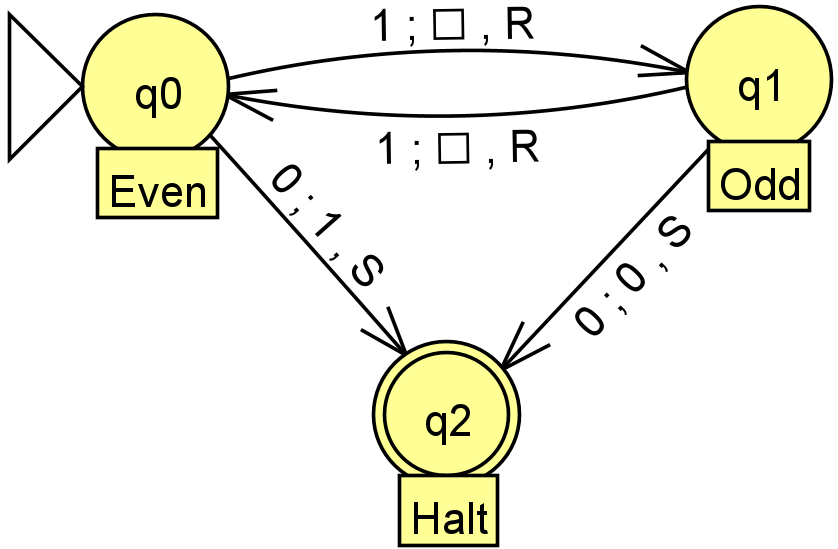
\includegraphics[width=10cm]{Images/SampleTMCrop.png}
       \caption{A TM that determines the cardinality of the length of a sequence of 1's on the tape.}
           \label{fig:TM}
\end{figure}

\subsection{Oracles}\label{subsec:Oracles}

Of course there also exists the Oracle, sometimes called Turing Machines with an oracle, which is capable of solving problems that TMs cannot.
It does so by having the ability to respond to any given problem from the TM it is connected to.
For example, the oracle would be able to solve the Halting Problem for the associated Turing Machine, but not the Halting Problem in general for all Turing Machines.
The reason the oracle is not considered more powerful is because in practice (i.e. reality), is because there is no such all-knowing source to retrieve information from.
As a result, I will disregard the Oracles for the rest of the thesis.

\subsection{Universal Turing Machines}\label{subsec:UTM}

A simple abstraction of the standard TM is a Universal Turing Machine. A UTM is capable of solving any computable problem, given the exact process/rules of the TM that will solve it.
In essence it is a machine that is not hard-coded with what to perform when given input.
The UTM will read the input, and respond based on the rules given.
As a result, the UTM is equivalently as powerful as a TM.
The only functional difference is the usability of the UTM towards a larger number of problems as opposed to the TM being created for a singular problem.

\subsection{The Church-Turing Thesis}\label{subsec:Church-Turing Thesis}

According to the Church-Turing Thesis, every effectively calculable function can be computed by a Turing Machine.
As explained by Robin Gandy, the main idea was to show that there is an upper bound on the computation of TMs.
This upper bound does not exist for humans and is therefore the basis of separation between computation power of TMs and humans.

\begin{thm}
    \label{thm:CTT}
    (Church-Turing Thesis) Every effectively calculable function can be computed by a Turing Machine.
\end{thm}

He proposed a series of four Principles that we still use today as a basis for determining what one of the definitions of a TM is capable of computing.
Any automata that violates any of these Principles is said to have "free will", which in context means being able to compute any non-computable function.
As an example, the Oracle machine would be capable of computing a non-computable function, namely the halting problem, and thus would have "free will".
We disregard such automata as there aren't any systems that exist in reality as of yet to display "free will".
As a result, TMs are the most powerful automata that can compute any calculable function.
This is why the Church-Turing thesis is generally assumed to be true \cite{GandyPaper}.

\subsection{Rice's Theorem}\label{subsec:RiceThm}

Another famous theorem to consider is Rice's Theorem.
It is widely known in the domain of computability theory as it defines the bounds of research in a formal manner.
Below is the Formal statement of Rice's Theorem, which will be supplemented with a concise statement summarizing the theorem \cite{WolframRiceThm,WikiRiceThm}.

\begin{thm}
    \label{thm:RiceThm}
    (Rice's Theorem) Let $\varphi$ be an admissable numbering of partial computable functions. 
    Let P be a subset of $\mathbb{Z}$.
    Suppose that:
    \begin{enumerate}
        \item P is non-trivial: P is neither empty nor $\mathbb{N}$ itself.
        \item P is extensional: $\forall  m,n \in \mathbb{N}$, if $\varphi_{m} = \varphi_{n}$,
        then $m \in P \Leftrightarrow n \in P$.
    \end{enumerate}
    Then P is undecidable.

    I.e. The only decidable index sets are $\emptyset$ and $\mathbb{N}$.
\end{thm}

This directly translates to programming languages as stating: All non-trivial smenatic properties of programs are undecidable.
Thus, Rice's theorem is a generalization of the Halting Problem.
Because of this theorem, it is impossible to design a program that determines if a given program is able to execute without error.
Another view of thie theorem is that it states only trivial properties of programs are algorithmically decidable.
Eg. If a program has an if statement inside the code.

\section{Turing Completeness}\label{sec:TC}

Turing Completeness is a closely related term when discussing Turing Machines.
For a system to be Turing Complete, it must be capable of performing any computation that a standard TM can perform.
An equivalent description would be that for a system to be TC, it must simulate a UTM.
By transitivity, if any system is proven to be TC, then it must be equivalent in power to all other systems that are TC.
Therefore, all TC systems are considered the most powerful computation machine.

\subsection{Considering the Practicality of Turing Complete Programming Languages}\label{subsec:PracticalTC}

Despite all TC systems being equivalent in computation power, this does not mean that all are practically useful.
This is because despite the TC being able to simulate any TM, it may have a more complex method for simulation or calculation of the same problem.
This is considered a non-issue as the length of time needed for computation is not considered when discussing TMs and TC systems.
This is only a factor for practical purposes, such as programming languages, space and time complexity are of major importance.

\subsubsection{Esoteric Progamming Languages}\label{subsubsec:EsotericPL}

Esoteric programming languages are designed to demonstrate a key concept with language design, but are often done so in a joking manner.
An example of a highly simplistic well-known esoteric TC language is brainfuck.
I will describe the way brainfuck operates and then provide several example programs with explanations.

The language has only 8 instructions, a data pointer, and an instruction pointer.
It uses a single dimensional array containing 30,000 byte cells, with each cell initialized to zero.
The data pointer points to the current cell within the array, initialized to index 0.
The instruction pointer points to the next instruction to be processed, starting from the first character given in the code.
Any characters besides those used in the instructions are considered comments and will be ignored.
Instructions are executed sequentially unless branching logic is taken via the '[' or ']' instructions.
The program terminates when the instruction pointer moves beyond the final command.
Additionally, it has two streams of bytes for input and output which are used for entering keyboard input and displaying output on a monitor using the ASCII encoding scheme \cite{BfWiki,BfGH}.

The 8 instructions are as follows:
\begin{table}[h!tb]
    \centering
    \begin{tabular}{|c|p{10cm}|}
        \hline
        \textbf{$>$} & Increments the data pointer by one. (This points to the next cell on the right). \\
        \hline
        \textbf{$<$} & Decrement the data pointer by one. (This points to the next cell on the left). \\
        \hline
        \textbf{$+$} & Increments the byte at the data pointer by one. \\
        \hline
        \textbf{$-$} & Decrements the byte at the data pointer by one. \\
        \hline
        \textbf{$.$} & Output the byte at the data pointer. \\
        \hline
        \textbf{$,$} & Accept one byte of input, storing its value in the byte at the data pointer.\\
        \hline
        \textbf{[} & If the byte at the data pointer is zero, then instead of moving the instruction forward to the next command, go to the matching ']' command. (Jump forwards). \\
        \hline
        \textbf{]} & If the byte at the data pointer is non-zero, then instead of moving the instruction forward to the next command, go to the matching '[' command. (Jump backwards). \\
        \hline
    \end{tabular}
    \caption{Brainfuck Instruction Set}
    \label{tab:BrainfuckInstructionSet}
\end{table}

Each '[' or ']' must correspond to match with it's complement symbol, namely ']' and '[' respectively.
Also, when input is read with the ',' command the given character from a keyboard input will have its value read as a decimal ASCII code
(eg. '!' corresponds to 33. 'a' corresponds to 97, etc.).
The decimal value is what is then converted to binary and stored within the current byte \cite{BfSO}.

Here is a simple program that modifies the value of the first cell in the 30,000 byte array.

\begin{verbatim}
    ++      Add 2 to the byte value in cell 0
    [-]     Decrement the value of the current cell until it reaches 0
\end{verbatim}

In fact, we can remove the comments and put the code onto a single line to achieve the same result.
Recall that comments include any character that is not listed as one of the 8 aforementioned instructions.

\begin{verbatim}
    ++[-]
\end{verbatim}

\newpage

An equivalent program in python is seen below:

\begin{verbatim}
    # Let 'Array' be our 30,000 byte array
    Array[0] += 2
    while (Array[0] != 0):
        Array[0] -= 1
\end{verbatim}

Below is an example program that outputs Hello World.
At the end of each line is the end result of the operations done in the line as a comment.
Each line prints a new character.

\begin{verbatim}
    >++++++++[<+++++++++>-]<.       H
    >++++[<+++++++>-]<+.            e
    +++++++..                       l
    +++.                            l
    >>++++++[<+++++++>-]<++.        o
    ------------.                   [space]
    >++++++[<+++++++++>-]<+.        W
    <.                              o
    +++.                            r
    ------.                         l
    --------.                       d
    >>>++++[<++++++++>-]<+.         !
\end{verbatim}

For an in-depth breakdown of brainfuck with examples and guiding logic like the one above, read: \cite{BfGH}.
One common technique utilized when creating programming languages is to bootstrap them.
This means that the developers will write a compiler for the language, using the language itself.
This is done for many reasons, but the reason for introducing it here is to show how brainfuck is capable of complex logic that is more practically useful than simple programs as seen above.
Below is the current smallest bootstrapped compiler for brainfuck \cite{SmallestBfCompiler,SmallestBfCompilerActual}.

\begin{verbatim}
    >>>+[[-]>>[-]++>+>+++++++[<++++>>++<-]++>>+>+>+++++[>++>++++++<<-]+>>>,
    <++[[>[->>]<[>>]<<-]<[<]<+>>[>]>[<+>-[[<+>-]>]<[[[-]<]++<-[<+++++++++>[
    <->-]>>]>>]]<<]<]<[[<]>[[>]>>[>>]+[<<]<[<]<+>>-]>[>]+[->>]<<<<[[<<]<[<]
    +<<[+>+<<-[>-->+<<-[>+<[>>+<<-]]]>[<+>-]<]++>>-->[>]>>[>>]]<<[>>+<[[<]
    <]>[[<<]<[<]+[-<+>>-[<<+>++>-[<->[<<+>>-]]]<[>+<-]>]>[>]>]>[>>]>>]<<[>>
    +>>+>>]<<[->>>>>>>>]<<[>.>>>>>>>]<<[>->>>>>]<<[>,>>>]<<[>+>]<<[+<<]<]
\end{verbatim}

As we quickly found out, using brainfuck in any practical sense is simply too much work due to its extreme inefficiency.
It also is extremely difficult to understand without comments indicating the goal of each step.
Due to the simplicity of the language, it is very useful for studying Turing Completeness.
There exist many other esoteric TC programming languages, but the reason for choosing brainfuck in particular is its simple instruction set.
As a result, we will now look at more useful and practical programming language paradigms.
These languages within these paradigms will be much more efficient and legible, at the cost of increased complexity in instruction set.

\subsubsection{Procedural Languages}\label{subsubsec:ProceduralPL}

Procedural Programming Languages are designed to be read linearly in execution order, top to bottom.
The main idea behind this design of languages is to create procedures and subprocedures (equivalently routines and subroutines), to achieve a larger goal.
For example to calculate the sum of squares in code you may design it in the C code as follows:

\begin{verbatim}
    float squareNumber(float a) {
        return a * a;
    }
    float findSumOfSquares (float a, float b) {
        return squareNumber(a) + squareNumber(b);
    }
\end{verbatim}
    
When working in Procedural Programming Languages, variables are used to store and modify data.
These variables may be locally or globally defined, which is where we define the concept of scope.
Scope refers to the current lens in which we view code and the system memory.
It identifies which variables exist, what values they have, and what operations are being performed.
The below example in C provides insight into the importance of scope.

\begin{verbatim}
    float globalVariable;

    float foo (float bar) {
        float localVariable;
        ...
    }

    float baz (float qux) {
        float localVariable;
        ...
    }
\end{verbatim}

Notice that we are able to utilize a variable named localVariable in the two functions foo and baz.
This is allowed because when the scope is inside of either function, the other function does not exist.
The variable globalVariable is available to both because it is outside of the scope of both functions.
This means that any other function in the code in the same scope as the globalVariable is capable of accessing its value.

I will now describe the importance of functions in Procedural Programming Languages.
Functions are designed to complete a single goal and return a single output.
They are capable of accepting a non-negative number of inputs and outputting 0 or 1 outputs.
These functions are capable of calling other functions, including themselves.
When a function calls itself, this is called recursion.
Here is an example constructing the fibonacci sequence in C in 2 ways: without recursion, and with recursion.

\begin{verbatim}
    //Given an integer n, calculate the first n numbers
    //of the fibonacci sequence without recursion
    
    void sequentialFibonacci (int n) {
        if (n < 1) {
            printf("Input must be an integer greater than 0");
                return;
        }

        int sub1 = 0;
        int sub2 = 1;

        for (int i = 1; i <= n; i+=1) {
            if (i > 2) {
                int curr = sub1 + sub2;
                sub1 = sub2;
                sub2 = curr;
                printf("%d ", curr);
            }
            else if (i == 1) {
                printf("%d ", sub1);
            }
            else if (i == 2) {
                printf("%d ", sub2);
            }
        }
    }

    /***************************************************************/

    //Recursive case

    //keep track of current Index, given amount of fibonacci numbers
    //to print, and propogate the two subnumbers to the next step
    void recursiveFibonacci (int currIndex, int n, int sub1, int sub2) {
        if (currIndex < n) {
            printf("%d ", sub1 + sub2);
            recursiveFibonacci(currIndex + 1, n, sub2, sub1 + sub2);
        }
        return;
    }

    //handle base cases (exit conditions)
    //otherwise start the recursive process
    void startRecursiveFibonacci (int n) {
        if (n < 1) {
            printf("Input must be an integer greater than 0");
        } else if (n == 1) {
            printf("%d ", 0);
        } else if (n == 2) {
            printf("%d %d ", 0, 1);
        } else {
            printf("%d %d ", 0, 1);
            recursiveFibonacci(0, n - 2, 0, 1);
        }
        return;
    }
\end{verbatim}

As shown above, recursion is a powerful tool to simplify the amount of lines needed to code the main functionality of the procedure.
It simplifies the amount of lines written because the overall logical design is more complex.

Through the use of scope and compartmentalizing procedures, Procedural programming is a very straightforward and capable design paradigm for software development.
Some well known languages that are Turing Complete from this paradigm are: 
\begin{itemize}
    \item C
    \item Pascal
    \item COBOL
    \item Fortran
    \item ALGOL
    \item Basic        
\end{itemize}

Although these languages are very old, with some coming from the 1960s, some still find modern use.
Linus Torvalds, the creator of the Linux kernel and git, chose C to be the main language for developing both of these well known pieces of software.
Both are still actively developed and improved to this day and remain majorly written in C \cite{GitMadeinC,LinuxMadeinC}.
Additionally, Richard Stallman led the development for the GNU operating system using C \cite{GNUPreferC}.
Although most users are on the Windows or Apple platform for PCs, the GNU operating system with the Linux kernel is still a popular choice amongst users looking for a different experience \cite{MarketShareOS}.
Besides C, COBOL remains a language that is used professionally for banking.
Many banks still use COBOL their business application and management \cite{COBOLBanks}.

\subsubsection{Object Oriented Languages}\label{subsubsec:OOPL}

A different scheme altogether for a programming language is an Object Oriented Language.
Developing in this language paradigm is known as a Object Oriented Programming.
OOP is structured entirely different than Procedural Programming.
Instead of defining procedures to solve the problem, we utilize a new idea of coding.
We outline classes, which are representations of some system that we wish to design.
Classes contain 3 parts: Data Members, Constructors, and Methods.
Data Members are used to describe what the Class is.
For example, if I want to model a school, an important data member would be the amount of students enrolled.
Constructors are ways to create an instance of the class.
This is where the object is created.
In the school example, perhaps there would be two ways to create a school: with a total amount of students enrolled already, and another without.
Both are valid as adding an existing school to the digital system would use the first constructor, while creating a new school would utilize the second constructor.
Methods are ways we modify the attributes of the objects.
Perhaps a certain amount of students enroll into the newly created school.
We must have a way to update the amount of students for any school.
These 3 parts form the basis of what OOP looks like.
Below is a snippet of Java code demonstrating these principles.

\begin{verbatim}
class School {
    private int numEnrolledStudents;
    
    public School () {
        this.numEnrolledStudents = 0;
    }
    
    public School (int numAlreadyEnrolled) {
        this.numEnrolledStudents = numAlreadyEnrolled;
    }
    
    public int getNumEnrolled() {
        return this.numEnrolledStudents;
    }
    
    public void setNumEnrolled(int numStudents) {
        this.numEnrolledStudents = numStudents;
        return;
    }
}

class RunCode {
    public static void main(String[] args) {
        School NewSchool = new School();
        
        System.out.println("The number of students enrolled 
            in the new school is: " + NewSchool.getNumEnrolled()); // 0
        
        NewSchool.setNumEnrolled(100);
        
        System.out.println("The number of students enrolled
            in the new school is: " + NewSchool.getNumEnrolled()); // 100
        
        School CSUN = new School(32172);
        
        System.out.println("The number of students enrolled
            at CSUN is: " + CSUN.getNumEnrolled());                // 32172
    }
}
\end{verbatim}

There are more advanced features such as Inheritance that allow for more complex design models.
Furthermore, Java contains Modifiers which are used to change the permission of which piece of code is capable of being accessed by another piece of code.
In the above example, only the school object is capable of managing the data of numEnrolledStudents \cite{CSUNStudents}.
Through the use of the methods getNumEnrolled and setNumEnrolled, any other class can modify the value of the class, but only through the reference of the school object.

Some well known languages that are Turing Complete from this paradigm are: 
\begin{itemize}
    \item Java
    \item C++
    \item Scala
    \item PHP
    \item Perl
    \item Swift        
\end{itemize}

%INSERT SECTION ON USE CASES HERE

\subsubsection{Multi Paradigm Languages}\label{subsubsec:MultiParadigmPL}

Some languages allow for the combination of OOP and Procedural Programming.
In such paradigms, the code allows for both to be run at the same time and enjoys the benefits of both approaches, at the cost of increased design overhead of the project.
Here is an example snippet of Python code that demonstrates both at the same time:

\begin{verbatim}
    def findSumOfSquares(num1, num2):
        return (num1 ** 2) + (num2 ** 2)

    class Homework:
        def __init__(self, problem):
            self.problem = problem
            
        def problem(self, problem):
            self.problem = problem

    HW = Homework("What is the sum of squares of 2 and 3?")
    print(HW.problem)

    print(findSumOfSquares(2, 3))

    #####       Printed to Terminal     #####

    What is the sum of squares of 2 and 3?
    13  
    
\end{verbatim}

In the code example, we utilize Procedural Programming to create the findSumOfSquares function.
Through the usage of OOP, we create a Homework object that has a single data member, a single problem.
By accessing the problem within the Homework object, we are able to print it out, then use the function to solve it.

Some well known languages that are Turing Complete from this paradigm are shown below.
Notice that some languages mentioned in the previous sections may show up in the list: 
\begin{itemize}
    \item JavaScript
    \item C++
    \item Python
    \item R
    \item Perl
    \item Fortran
\end{itemize}

Multi Paradigm languages have a lot of flexibility for the applications that they can be used to create.
The top frontend frameworks for web development use Javascript as their main language including React, Vue, Svelte, and more \cite{JSPopular}.
Python is very popular for its legible and flexible code.
With its libraries such as Tensorflow and Keras, Machine Learning and other AI subgenres are easier to implement than in other languages.
The popular LLM ChatGPT is primarily written in python \cite{ChatGPTPython}.
R is another language that is popular for its data science capabilities.
It is heavily used within the sciences (alongside python) because of its simplistic syntax, as well as its numerous libraries for data analysis \cite{RDataSci,DataSciLangs}.

%%%%%%%%%%%%%%%%%%%%%%%%%%%%%%%%%%%%%%%%%%%%%%%%%%%%%%%%%%%%%%%%%%%%%%%%%%%%%%%%%%%%%%%%%%%%%%%%


% \subsubsection{Functional Programming Languages}

% Consider these next two sections as an outline and series of notes on what to do.
% They aren't fleshed out like the rest of the document that is written.

% NOT SURE IF I WANT TO KEEP THE FOLLOWING 2 SECTIONS OR NOT: FUNCTIONAL PROGRAMMING LANGUAGES, LOGIC PROGRAMMING LANGUAGES.
% I WOULD PROBABLY KEEP IT SIMPLE WITH 1-3 THINGS TO DESCRIBE ABOUT THE WAY THE LANGUAGE IS STRUCTURED W/ 1-2 CODE EXAMPLES AND EXPLANATIONS.
% (I ESTIMATE 3-5 PAGES PER SECTION DEPENDING ON SIZE OF EXAMPLES).
% I THINK I'VE SHOWN MY POINT, WHICH IS THAT THE DIFFERENT PARADIGMS ARE CAPABLE OF BEING TC DESPITE BEING SO DIFFERENT FROM EACH OTHER.
% IT MIGHT BE COOL/INTERESTING TO SHOW THE DIFFERENT THINKING INVOLVED FOR LANGUAGES LIKE PROLOG.
% I COULD ALSO COME BACK TO ACKNOWLEDGE CERTAIN ASPECTS OF LANGUAGE DESIGN PRINCIPLES HERE, WHICH WOULD REQUIRE FURTHER READING.
% I DO ADMIT THAT THIS IS SOMEWHAT OUTSIDE THE SCOPE OF THIS THESIS BECAUSE IM NOT EXACTLY LOOKING AT THE STYLE OF LANGAUGE OF PROTEUS, NOR HOW IT COMPARES TO THESE PARADIGMS TO CATEGORIZE IT.

% describe design of these languages
% Some well known languages that are Turing Complete from this paradigm are:  
% \begin{itemize}
%     \item Lisp
%     \item Haskell
%     \item Elixir
%     \item OCaml
%     \item Scala
% \end{itemize}

% DESCRIBE SOME ACTUAL USAGE OF THESE PROGRAMS IN MODERN SOFTWARE DEVELOPMENT

% RUST IS BEING USED TO TRY TO CREATE A NEW AND DIFF LINUX KERNEL.
% GO IS NEW POPULAR PROGRAMMING LANGUAGE FOR WEB DEVELOPMENT, DEVOPS, ETC.

%%%%%%%%%%%%%%%%%%%%%%%%%%%%%%%%%%%%%%%%%%%%%%%%%%%%%%%%%%%%%%%%%%%%%%%%%%%%%%%%%%%%%%%%%%%%%%%%

\section{Proteus}\label{sec:Proteus}

The main goal of this thesis is to outline a proof demonstrating that a novel prototype language, Proteus, is TC.
In this section, I will describe in detail what Proteus is.

\subsection{Proteus Description}\label{subsec:ProteusDescription}

Proteus is a programming language and compiler being developed as a project for CSUN's Autonomy Research Center for STEAHM in collaboration with the NASA Jet Propulsion Laboratory (JPL).
JPL system engineers needed a safer language to develop autonomous systems reliably, which is why Proteus was created.
Proteus allows for the creation of different models: actors and hierarchical state machines.
It is compiled to C++ with the C++17 standard \cite{ProteusRunTime}.

Proteus is a programming language that follows the Actor model paradigm, which is somewhat related to the OOP paradigm.
The difference lies in that Actor model allows for concurrent computation, while OOP generally runs sequentially.
This means that parallelism is inherently existent in the language \cite{ActorModelParallel,ActorJavaParallel}.
Furthermore, because of the design of the events and event queue for Actors, any code involving them is run sequentially.
This means that Proteus also supports the Procedural Programming langauge paradigm.
Thus, Proteus is a Multi Paradigm language that enjoys the ability to utilize features such as scope, recursion, and so forth.

\subsubsection{Actors}\label{subsubsec:Actors}

Actors are independent entities within concurrent systems.
By allowing several actors to operate independently, there is: no sharing of resources, concurrent runtime, and only interact amongst each other via a message system.
Communication is asynchronous because the messages get buffered by the system until the recipient can handle them.
Actors can send messages, modify local state, or create more actors based on the message handling.

\subsubsection{Hierarchical State Machines}\label{subsubsec:HSM}

Hierarchical State Machines allow developers to model the system that they are developing for.
These HSMs are an extension to the standard definition of a state machine as HSMs allow states to be HSMs themselves.
This allows for simplification of the states and transitions amongst states allowing simpler models for usage in the real-world.

Actors have a non-negative amount of associated HSMs while each HSM belongs to exactly one actor.
Event Handlers are the way that messages are sent amongst machines as well as how the machine perform state transitions.
Actors and states are statically defined, which means that they cannot be created nor destroyed at runtime.
When compiled, Actors and states are created as C++ structs.

\subsection{Proteus Grammar}\label{subsec:ProteusGrammar}

Below is the Grammar for Proteus.
It outlines the command followed by the definition for writing the command.
Anything outlined in single quotations indicates text to be written explicitly.
It is to be read as: 'OPERATION' can be written as 'HOW TO WRITE THE OPERATION'.

\begin{verbatim}
Program: DefEvent* DefGlobalConst* DefFunc* DefActor+
DefActor: 'actor' ActorName '{' ActorItem* '}'
ActorItem: DefHSM | DefActorOn | DefMember | DefMethod
DefActorOn: 'on' EventMatch OnBlock
DefHSM:   'statemachine' '{' StateItem* '}'
DefState: 'state' StateName '{' StateItem* '}'
StateItem: DefOn | DefEntry | DefExit | DefMember | 
            DefMethod | DefState | InitialState
DefOn: 'on' EventMatch OnBody
EventMatch: EventName '{' [VarName (',' VarName)*] '}'
OnBody: GoStmt | OnBlock
OnBlock: Block
DefEntry: 'entry' '{' Block '}'
DefExit: 'exit' '{' Block '}'
DefMember: Type VarName '=' ConstExpr ';'
DefMethod: 'func' FuncName FormalFuncArgs ['->' Type] Block
InitialState: 'initial' StateName ';'
Block: '{' Stmt* '}'
Stmt: IfStmt | WhileStmt | DecStmt | AssignStmt | ExitStmt | 
            ApplyStmt | SendStmt | PrintStmt | PrintlnStmt
DefEvent: 'event' EventName '{' [Type (',' Type )*] }' ';'
DefFunc: 'func' FuncName FormalFuncArgs ['->' Type] Block
DefGlobalConst: 'const' Type VarName '=' ConstExpr ';'
ExitStmt: 'exit' '(' NUMBER ')' ';'
ReturnStmt: 'return' Expr ';'
DecStmt: Type VarName '=' Expr ';'
AssignStmt: VarName '=' Expr ';'
ApplyStmt: ApplyExpr ';'
SendStmt : HSMName '!' EventName ExprListCurly ';'
PrintStmt : 'print' ExprListParen ';'
PrintlnStmt : 'println' ExprListParen ';'
FormalFuncArgs : '(' [Type VarName (',' Type VarName)*] ')'
ExprListParen :'(' [Expr (',' Expr)*] ')'
ExprListCurly :'{' [Expr (',' Expr)*] '}'
Type: 'int' | 'string' | 'bool' | 'actorname' | 'statename' | 
            'eventname'
GoStmt: JustGoStmt | GoIfStmt
JustGoStmt: 'go' StateName Block
GoIfStmt: 'goif' ParenExpr StateName Block 
            ['else' (GoIfStmt | ElseGoStmt)]
ElseGoStmt: 'go' StateName Block
IfStmt: 'if' ParenExpr Block ['else' (IfStmt | Block)] 
WhileStmt: 'while' ParenExpr Block 
ParenExpr: '(' Expr ')' 
ConstExpr: IntExpr | BoolExpr | StrExpr
Expr: ValExpr | BinOpExpr | ApplyExpr
BinOpExpr: ValExpr BinOp Expr 
BinOp: '*' | '/' | '%' | '+' | '-' | '<<' | '>>' | '<' | '>' |
            '<=' | '>=' | '==' | '!=' | '^' | '&&' | '||' | '*=' | 
            '/=' | '%=' | '+=' | '-=' | '<<=' | '>>=' | '^='
ApplyExpr: FuncName ExprListParen
ValExpr: VarExpr | IntExpr | StrExpr | BoolExpr | ActorExpr | 
            StateExpr | EventExpr | ParenExpr
VarExpr: VarName
IntExpr: NUMBER 
StrExpr: STRING 
BoolExpr: BOOL
ActorExpr: 'actor' ActorName
StateExpr: 'state' StateName
EventExpr: 'event' EventName
StateName: NAME
ActorName: NAME
FuncName: NAME
VarName: NAME
EventName: NAME
\end{verbatim}

Looking at the grammar is similar to looking at the pieces of a puzzle without actually arranging the pieces together.
Below is an example written in Proteus code that showcases Actors and HSMs in a system.

There are a total of 3 events: POWER\_ON which accepts a boolean as input, POWER\_OFF, and NEXT with the latter two not accepting an inputs.
There are 2 actors: Main and Driver.
Main has a single state machine with 2 states: On and Off.
Main defines an internal boolean for whether Mode2 is enabled.
By default it is initialized to false.
The HSM within Main is initalized to Off, and switches to On when the POWER\_ON event is registered.
Furthermore, it updates the value for Mode2 being enabled with the input for POWER\_ON.
When turned On, there is a defined Mode1 that is the initial mode of the machine.
It then defines what the machine does when it is turned on and off.
In both cases, it outputs a message indicating the status of the power state of the machine (on prints on, and off prints off).
Mode1 prints to the output the current Mode, and then has logic determining what to do when the NEXT message is received.
If the machine has mode2\_enabled set to true, then it should should go to Mode2.
Mode2 simply prints the current mode when it is entered.
The second actor is the Driver.
It determines the actions to be taken by Main in a series of messages (events) that are broadcasted from its internal statemachine.
Upon turning on the machine, it will send the event for Main to turn on with an input of true.
Then it sends Main the NEXT event twice.
It then tells Main to power off with the POWER\_OFF event.

\begin{verbatim}
event POWER_ON {bool};
event POWER_OFF {};
event NEXT {};
actor Main {
    bool mode2_enabled = false;
    statemachine {
        initial Off;
        state Off {
            on POWER_ON {x} {go On {mode2_enabled = x;}}
        }
        state On {
            initial Mode1;
            entry {println(“turning on”);}
            exit {println(“turning off”);}
            on POWER_OFF {} {go Off {}}
            state Mode1 {
                entry {println(“mode 1”);}
                on NEXT {} {goif(mode2_enabled) {Mode2 {}}}
            }
            state Mode2 {
                entry {println(“mode 2”);}
            }
        }
    }
}
actor Driver {
    statemachine {
        entry {
            Main ! POWER_ON {true};
            Main ! NEXT {};
            Main ! NEXT {};
            Main ! POWER_OFF {};
        }
    }
}
\end{verbatim}

From the above example, we can see the OOP and Procedural Programming properties that Proteus is capable of.
In fact, we can see the property of scope in action.
The local variable mode2\_enabled is only accessible within Main and the HSM within Main.
Furthermore, we see that the order of events is run in sequence.
Main accepts these events in the order received in the internal event queue, and is capable of responding based on the internal state conditions as well as the event received.
When this code is run, the output is seen below:

\begin{verbatim}
    turning on
    mode1
    mode2
    mode1
    turning off
\end{verbatim}

The goal of this Thesis is to analyze this language to prove that it is TC.
This is done by looking at the grammar and type of programming paradigm.
With this understanding, we will also look at different approaches for proving Turing Completeness.
Afterwards, we will demonstrate that Proteus is in fact turing complete using some of the methods seen in the next chapter.
    \chapter{Different Approaches for Proofs to Demonstrate Turing Completeness}\label{chapter:ProofApproachesForTC}

\section{Overview}\label{sec:ProofOverview}

We will be exploring the different approaches to demonstrate TC for different systems.
I have outlined the approaches based on their respective discipline, increasing in abstraction.
With each discipline comes a more theoretical view and understanding of TMs and TC systems.
My intention is to add clarity on the logic for these proofs/techniques.
For example, in the Computer Engineering perspective, TM is created from its mechanical properties through the usage of logic gates.
This is vastly different compared to how Mathematicians show TC, which is through the use of Lambda calculus -- a model for representing mathematical logic.
All proofs are equivalent in goal, however.
These are not the only perspectives and types of proofs for showing Turing Completeness as well as TMs.
This is simply a survey into what TMs and Turing Completeness looks like across the disciplines.

\section{Computer Engineering}\label{sec:CE}

In this section, we will analyze what a TM looks like from a physical perspective.
This may seem contradictory because the TM is described as a theoeretical machine.
But in fact, the very computers that we use today are are capable of processing TC systems through the usage of programming languages.
This means that they are limited TMs, because they are bounded only in memory.
In this approach, we will look at the core components of Computer Engineering to create a TM.

\subsection{Logical Design of a TM}\label{subsec:TMLogicalDesign}

To define what a TM does, we must explore what it is capable of.
Recall Theorem \ref{thm:CTT} in \ref{subsec:Church-Turing Thesis}, "Every effectively calculable function can be computed by a Turing Machine."
Every effectively calculable function, as Turing and Church understood, was any mathematical calculation.
This means that a TM must have some ability to perform any operation on numbers, such as the basic operations of addition, subtraction, multiplication, and division.
Furthermore, they must be capable of combining these together to form more complex operations such as exponential arithmetic.
Beyond the mathematical aspect, they must allow for some sort of logic handling.
[BIOLOGY PAPER ON TM]

\subsubsection{Architecture}\label{subsubsec:Arch}

Looking at modern day computer architecture, there are several components that work independently but operate concurrently.
It is based off of the Modified Harvard Structure which is a variation of the Harvard computer architecture and Von Neumann architecture.
It combines both approaches towards computer architecture to handle many tasks that were difficult to handle using one of either architecture.

The von Neumann Architecture which has a centralized CPU to handle tasks for the computer.
All processes are handled by the CPU directly.
It contains several parts inside for processing data.
Inside the CPU is an ALU with registers, as well as a Control Unit.
The ALU processes arithmetic and logical computation, with the assistance of registers to store data at each step.
The Control unit determines the commands to be given to the ALU and other parts of the computer.
There is an associated Memory Unit which is where the bulk of memory storage lies.
Outside of the CPU are the Input and Output devices.

\begin{figure}[htb]
    \centering
    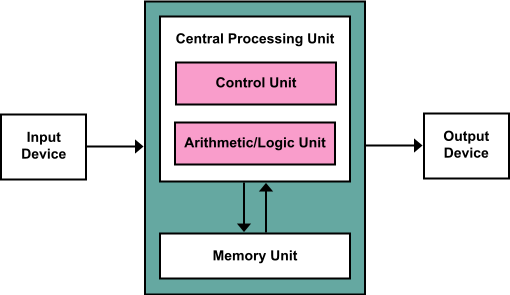
\includegraphics[width=10cm]{Images/Von_Neumann_Architecture.png}
       \caption{Von Neumann architecture.}
           \label{Fig:VonNeumannArch}
\end{figure}

\href{https://commons.wikimedia.org/wiki/File:Von_Neumann_Architecture.svg}{citation for von neumann architecture image}

The von Neumann architecture has several limitations, with one of the biggest criticisms being that it is bottlenecked by the throughput between the CPU and memory.
Essentially, the CPU will eventually have more processing power than the bus can handle to write/read from memory.
This causes the CPU to wait until the bus is freed to continue processing.
As an alternative, we will now look at the Harvard Architecture

The Harvard architecture looks at the problem as says that if the CPU is too large and complex, then each individual component should be separated.
This allows for the tasks to be distributed evenly amongst the several smaller components like the ALU and Instruction memory as opposed to having them live inside the CPU.
The CPU is capable of simultaneous reads and writes.
However, a similar bottleneck occurs where the bus connecting each of the components is the limiting factor.
Below is a diagram demonstrating the Harvard Architecture.

\begin{figure}[htb]
    \centering
    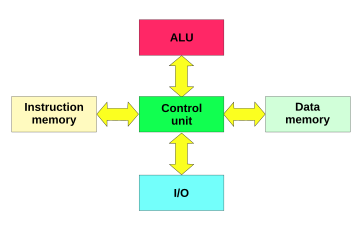
\includegraphics[width=10cm]{Images/Harvard_architecture.svg.png}
       \caption{Harvard architecture.}
           \label{Fig:HarvardArch}
\end{figure}

\href{https://commons.wikimedia.org/wiki/File:Harvard_architecture.svg}{citation for harvard architecture image}

However, modern day computers utilize a mixed computer architecture called the Modified Harvard architecture.
It combines both architectures into a single model.
This usually is of the form of separating the components of the computer, but allowing several smaller memory caches for the CPU.
This is why modern computers utilize several components such as the CPU, GPU, Main Memory (SDD or HDD) and so forth.
Furthermore, this advancement allows for paralellism or multi-core systems to arise.
Some notable examples include the NVIDIA RTX 4080 which has over 8000 cores \href{https://www.techpowerup.com/gpu-specs/geforce-rtx-4080.c3888}{SOURCE} or for the intel i9-13900ks CPU to have 16 cores \href{https://www.intel.com/content/www/us/en/products/sku/232167/intel-core-i913900ks-processor-36m-cache-up-to-6-00-ghz/specifications.html}{SOURCE}.
By allowing each one to independently operate, but still have the CPU as the "brains" of the operation.
We will now dive slightly deeper into the discussion to see what lies beneath these components within modern computer systems.

\subsubsection{Logic Gates}\label{subsec:LogicGates}

The basic building blocks for devices such as the ALU, CPU, and such are logic gates.
These are simplistic logical components that allow for processing of data and performing operations on them.

The core of the CPU relies on the ALU.
The ALU is contains registers which simply hold data inside.
Registers are associated with an address for referencing purposes.

Within the ALU there are smallers components that perform specific operations such as addition and subtraction.
These smaller components utilize logical gates such as the OR gate to compute the result with the given input.
See the example below for a 2-Bit ALU that can process OR, AND, XOR, and addition calculations.

\begin{figure}[htb]
    \centering
    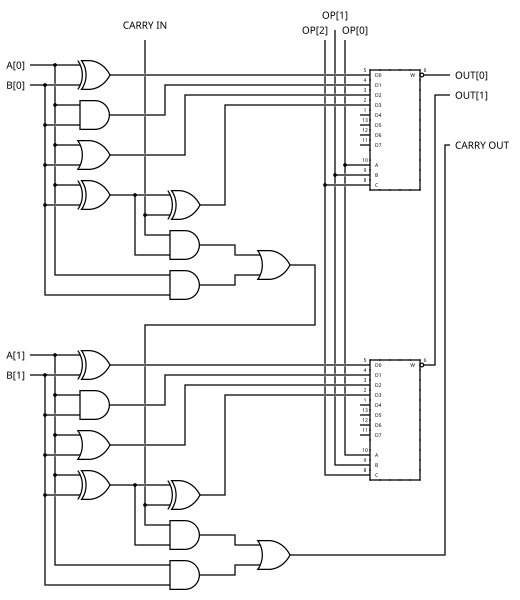
\includegraphics[width=10cm]{Images/2-bit_ALU.svg.png}
       \caption{A 2-Bit ALU.}
           \label{Fig:2BitALU}
\end{figure}

\href{https://en.wikibooks.org/wiki/File:2-bit_ALU.svg}{img src}

\subsection{Constructing the TM}\label{subsec:CreateTM}

With the ability to construct logic gates, we can create more complex components such as the ALU, CPU, and more.
Accompanied with the ability to store memory, as well as have a way to interact with the system through Input and Output, we are able to create a functional computer.
In the following examples, developers have successfully created computers in the well-known video games of Minecraft and Terraria respectively,
\href{https://www.youtube.com/watch?v=CW9N6kGbu2I}{Computer in Minecraft}
\href{https://www.youtube.com/watch?v=zXPiqk0-zDY}{Computer in Terraria}.
In fact, we will see later on that the computer built inside Terraria is verifiably TC via a method discussed in \ref{subsubsec:CGoL}.

This means that to construct a TM on a physical level (of course alleviating the restriction of unbounded memory), these would be the minimum requirements.

SRC - https://www.nand2tetris.org/
\href{https://www.amazon.com/Elements-Computing-Systems-Building-Principles/dp/0262640686/ref=ed_oe_p}{SRC - }

\section{Computer Science}\label{sec:CompSci}

In this section, we will conceptualize what a TM looks like under the lens of Computer Science.
There are 2 main perspectives: that of the Automata Theory and the Software Engineering approach.
The Automata Theory approach utilizes theoretical designs more reminiscent of those listed by Turing and Gavin.
The Software Engineering approach instead applies it to a problem to showcase Turing Completeness via programs and code.

\subsection{Automata Theory}\label{subsec:AutomataThy}

We will now abstract from the physical understanding of how to create a TM, to creating a theoretical one using Automata theory.
In automata theory, Turing Machines are described using logical notation.
The definition of a TM is stated within \cite{IntroFormLangAuto} and \cite{TuBB}.

\begin{definition}
    A Turing Machine $M$ is defined by:
        \[M = (Q, \Sigma ,\Gamma, \delta, q_{0}, \raisebox{0.1cm}{\fbox{}}, F)\]
        \par \hangindent=3cm \hangafter=1
        where: \\
        \( Q \) is the set of internal states,\\
        \( \Sigma \) is the input alphabet,\\
        \( \Gamma \) is the finite set of symbols called the tape alphabet,\\
        \( \delta \) is the transition function,\\
        \( \raisebox{0.1cm}{\fbox{}} \in \Gamma \) is a special symbol called the blank,\\
        \( q_{0} \in Q \) is the initial state,\\
        \( F \subseteq Q \) is the set of final states.
\end{definition}

The transition function $\delta$ is defined as \[\delta: Q \times \Gamma \rightarrow Q \times \Gamma \times \{L, R, S\}.\]
This means that for a given $\delta$ transition with inputs $q \in Q$ and $a \in \Gamma$, the tape will move to another state $x \in Q$, write nothing to the tape (indicated by \raisebox{0.1cm}{\fbox{}}) or some symbol $y \in \Gamma$, and choose to move the tape head Left one cell, Right one cell, or to Stay at the current cell.
An example transition can be written: \[\delta(q_{0}, a) = (q_{1}, d, R)\] where the internal state is $q_{0}$, and we read input token a.
After the transition, we have internal state $q_{1}$, wrote symbol d onto the tape, and moved to the right one cell.
See the below diagram demonstrating this change:

\begin{figure}[htb]
    \centering
    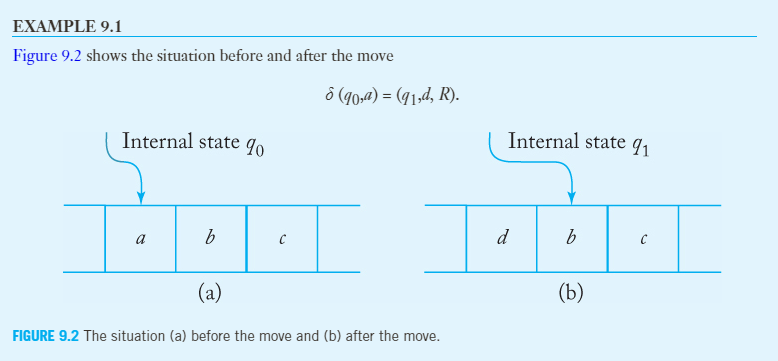
\includegraphics[width=16cm]{Images/deltatransition.png}
       \caption{Delta transition example from \cite{IntroFormLangAuto}.}
           \label{Fig:DeltaTransition}
\end{figure}

Recall Figure \ref{Fig:TM} which represents a simplistic TM.
In formal nomenclature, it can be written as follows:
\[
    \begin{aligned}
        Q &= \{q_{0}, q_{1}, q_{2}\} \text{ with associated labels \{Even, Odd, Halt\}}\\
        \Sigma &= {0,1}\\
        \Gamma &= {0,1}\\
        F &= \{q_{2}\}\\
        q_{0} &\in \text{ Q as the initial state}
    \end{aligned}
\]
and
\[
    \begin{aligned}
        \delta (q_{0}, 0) &= (q_{2}, 1, S),\\
        \delta (q_{0}, 1) &= (q_{1}, \raisebox{0.1cm}{\fbox{}}, R),\\
        \delta (q_{1}, 0) &= (q_{2}, 0, S),\\
        \delta (q_{1}, 1) &= (q_{0}, \raisebox{0.1cm}{\fbox{}}, R).\\
    \end{aligned}
\]

\subsubsection{Notable examples using Formal language}

The proofs constructed using formal language usually modify the given system to meet these requirements.

In "Magic: the Gathering is Turing Complete", the authors modified the way the game is understood between 2 players.
They make the system force moves through clever leverage of the cards and their functions within the game \cite{MtGTC}.

In a different paper, "Turing Completeness and Sid Meier's Civilization", the system was also creatively modified to demonstrate Turing Completeness.
In each game, they constructed UTMs by utilizing the layout of the maps, as well as mechanics for changing states of the roads within the game \cite{CivTC}.

To show that Java Generics are TC, the authors showed that by creating a subtyping machine, it corresponds to only a small portion of the Java Generics while simulating TMs.
Following this discovery, they simulate a TM and then show that the given inputs are undecidable \cite{JavaGenericsTC}.
I.e. leveraging an extension of Rice's Theorem, see \ref{RiceThm}.

The idea of describing the system as a TM and showing it has an undecidable input is a common practice.
This technique is also seen in a paper titled "The Game Description Language is Turing Complete" \cite{GDLTC}.

\subsection{Software Implementation}\label{subsec:SoftwareImplementation}

As opposed to the various theoretical approaches seen previously in section \ref{subsec:AutomataThy}, this section outlines a different perspective.
Instead of constructing a TM within the compounds of the system, an equivalent proof is to implement a program that demonstrates TC.
By implementing any known TC program successfully implies that the overall system is TC.

One such implementation would be to create a functional example of a known TC cellular automata.
Cellular automata are models of computation which use grids of cells.
Each cell contains a finite number of states, belonging to only one at any given time.
There are rules that determine what state a cell should become.
These rules are applied to all cells simultaneously, and thus form the next step in the sequence.
These steps are made sequentially to show the changes over time.
This makes all cellular automata 0-player games, meaning after an initial configuration there is no further input from the user.
With the work from Stephen Wolfram and other researchers such as Matthew Cook, some of these rules of cellular automata have been shown to be TC.
Famous examples of cellular automata include Conway's Game of Life and Rule 110.

https://mathworld.wolfram.com/CellularAutomaton.html
\href{https://en.wikipedia.org/wiki/Cellular_automaton}{wiki cell automata} 

Cellular automata are sorted into 4 classes:
\begin{itemize}
    \item Class 1: Nearly all initial patterns evolve quickly into a stable, homogenous state.
    Any randomness in the initial pattern disappears.
    \item Class 2: Nearly all initial patterns evolve quickly into stable or oscillating structures.
    Some of the randomness in the initial pattern may filter out, but some remains.
    Local changes to the initial pattern tend to remain local.
    \item Class 3: Nearly all initial patterns evolve in a pseudo-random or chaotic manner.
    Any stable structures that appear are quickly destroyed by the surrounding noise.
    Local changes to the initial pattern tend to spread infinitely.
    \item Class 4: Nearly all initial patterns evolve into structures that interact in complex and interesting ways, with the formation of local structures that are able to survive for long periods of time.
    Class 2 type stable or oscillating structures may be the eventual outcome, but the number of required to reach this state may be very large, even when the initial pattern is realtively simple.
    Local changes to the initial pattern may spread indefinitely.
\end{itemize}

Wolfram conjectured that many class 4 cellular automata are capable of universal computation.
Both Conway's Game of Life and Rule 110 exhibit "Class 4 behavior" and have been proven to be Turing Complete \cite{CGoLTM}.

\href{https://en.wikipedia.org/wiki/Cellular_automaton#Classification}{Wiki src}
SRC - Cellular Automata: A Discrete Universe by Andrew Ilachinski

\subsubsection{Conway's Game of Life}\label{subsubsec:CGoL}

Conway's Game of Life is a 2D grid of cells extending infinitely in the x and y directions.
Each cell contains only 2 states: Alive (On) or Dead (Off).
The rules of CGoL are simple:

\begin{enumerate}
    \item Any live cell with fewer than two live neighbors dies. (Underpopulation)
    \item Any live cell with two or three live neighbors lives on to the next generation. (Survival)
    \item Any live cell with more than three live neighbors dies. (Overpopulation)
    \item Any dead cell with exactly three live neighbors becomes a live cell. (Reproduction)
\end{enumerate}

They are demonstrated in the following graphic:

\begin{figure}[h!]
    \centering
    \includegraphics[width=10cm]{images/cgol.png}
       \caption{rules of conway's game of life visualized}
           \label{fig:cgolrules}
\end{figure}

\href{https://www.quantamagazine.org/maths-game-of-life-reveals-long-sought-repeating-patterns-20240118/}{src for graphic}

CGoL is considered undecidable.
This is because given any initial pattern and a desired pattern at some later generation, there is no algorithm to determine whether the desired pattern will exist.
As such, it is analogous to the Halting Problem.

\subsubsection{Rule 110}\label{subsubsec:Rule110}

Whereas CGoL is created on a 2D plane, Rule 110 lives in the 1D space.
There is an infinite tape of cells that each may exist in one of two states: 0 or 1.
By looking at three cells in series, one can find what the next state of the middle cell will be.
Below are the rules for Rule 110:

\begin{enumerate}
    \item 111 makes 0
    \item 110 makes 1
    \item 101 makes 1
    \item 100 makes 0
    \item 011 makes 1
    \item 010 makes 1
    \item 001 makes 1
    \item 000 makes 0
\end{enumerate}

Here is an associated graphic:

\begin{figure}[htb]
    \centering
    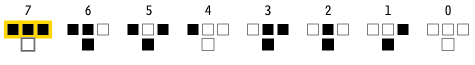
\includegraphics[width=10cm]{images/rule110.png}
       \caption{Rules for Rule 110}
           \label{fig:Rule110}
\end{figure}

Rule 110 is one of the simplest TC system that is known.
This makes it a relatively easy system to create to demonstrate Turing Completeness as opposed to CGoL.

\href{https://commons.wikimedia.org/wiki/File:One-d-cellular-automaton-rule-110.gif}{SRC - WIKI page for graphic}

\subsubsection{Programmable Calculator}\label{subsubsec:ProgCalc}

An entirely different approach to create a program that demonstrates Turing Completeness is to model the behavior of TMs directly.
This means that you create a system that does everything that a TM can do.
Recalling the Church-Turing Thesis (Theorem\ref{thm:CTT}), it must be able to calculate any function.
In a basic sense, this means that the system is capable of:

\begin{itemize}
    \item Reading/Writing memory
    \item Elementary Arithmetic/Logical operations
    \item Conditional Logic
    \item Looping Logic
\end{itemize}

Programmable Calculators meet all of these requirements.
By being able to store values into variables which can be referenced later, it can read/write memory.
Because it is a calculator, it is capable of performing arithmetic operations.
If statements and while loops are sufficient for handling the conditional and looping logic.
A programmable calculator thefore is TC.

A simplistic set of steps is outlined below:

\begin{enumerate}
    \item Start by making a basic arithmetic calculator.
    \item Then add the ability to store values into variables.
    \item Afterwards, create functionality for if statements, allowing boolean logic.
    \item Finally, create looping logic with while statements.
\end{enumerate}

\href{https://www.youtube.com/watch?v=_Uoyufkb5lk}{TC language in Ruby using Bable-Bridge}

This much simpler approach is easier to digest and reason out with some software engineering design principles.

\subsubsection{Interpreter for a known Turing Complete language}\label{subsec:InterpreterTC}

Alternatively, to show a programming language is TC, one can create an interpreter for a known TC language.
Many programming languages feature complex grammars and rulesets, which is why TC esoteric programming languages are preferred.
In fact brainfuck, as seen in section \ref{subsubsec:EsotericPL}, is used to demonstrate TC for its concise ruleset.

c bf interpreter: https://thesharperdev.com/how-to-write-a-brainfuck-interpreter-in-c/

novel lang meep that compiles to bf and thus is TC: https://github.com/srijan-paul/meep
https://injuly.in/blog/bfinbf/index.html

python bf interpreter: https://martin-ueding.de/posts/creating-a-brainfuck-interpreter/


\section{Mathematics}\label{sec:Maths}

In this section, I will take a look at the mathematical system that is most well known for being TC, Lambda Calculus.
This is an abstract form of understanding functions and their capabilities.
It was actually designed by Church, and proven to be TC later on based off the work of Turing and Church by a famous mathematician: Stephen Cole Kleene \cite{LambdaCalcKleene}.

\subsection{Lambda Calculus}\label{subsec:LambdaCalc}

Lambda calculus upon initial inspection seems like a very abstract form of functions and relations within mathematics.
It can be understood to those in Computer Science as a very abstract programming language, and actually forms the basis of Functional Programming Languages \cite{TutLambdaCalc}.
\href{https://learn.saylor.org/mod/book/tool/print/index.php?id=33044&chapterid=13087}{SRC - functional programming}.

Lambda Calculus is a form of expressing functions in a simple manner that allows for creating any complex system \cite{LambdaCalcRG}.
At its core, it consists of three inductive rules defining what lambda terms are.
Each lambda term is a valid statement in lambda calculus:
\begin{enumerate}
    \item \textit{x}: A \textbf{variable} to represent a character or string.
    This is to be understood as a parameter for functions.
    \item \textit{$\lambda x.M$}: A lambda \textbf{abstraction} that is a function definition.
    This function takes the bound variable \textit{x} as input, and returns the body \textit{M}.
    \item \textit{(M N)}: An \textbf{application} where it applies the function \textit{M} to argument \textit{N}.
\end{enumerate}

There also exist reduction operations to improve legibility but retain equivalent logical meaning:
\begin{enumerate}
    \item \textit{($\lambda x.M[x]$) $\rightarrow$ ($\lambda y.M[y]$)}: $\alpha$-conversion, which renames the bound variables in the expression.
    This is be used to avoid name collisions.
    \item \textit{(($\lambda x.M$)\textit{N}) $\rightarrow$ ($M[x:=N]$)}: $\beta$-reduction, which replaces bound variables with the argument expression in the body of the abstraction.
    This is used to simplify chained functions being written out.
\end{enumerate}

Parentheses may be used to to disambiguate terms from each other.
This is especially useful when constructing complex applications using lambda calculus.

\href{https://en.wikipedia.org/wiki/Lambda_calculus}{SRC - Lambda Calculus wiki}

I will define an equivalent TM to the previously mentioned TM seen in Figure \ref{Fig:TM} and in section \ref{subsec:AutomataThy}.
Recall that the goal of the TM was to determine if there are an even or odd number of '1's in a sequence.

We construct the list of Natural Numbers, $\mathbb{N}$, as follows:
\[
    \begin{aligned}
        0 &\equiv \lambda sz.s(z)\\
        1 &\equiv \lambda sz.s(s(z))\\
        2 &\equiv \lambda sz.s(s(s(z)))\\
        &\text{and so on...}\\
    \end{aligned}
\]

Now we construct the ideas of Arithmetic Boolean Logic, and other necessary logical operators.
Treat 'f' as a function and variables as only locally defined to their respective operator.
These examples can be seen here: \href{https://jwodder.freeshell.org/lambda.html}{SRC}.
Some notation can be interpreted as SKI combinator calculus \href{https://en.wikipedia.org/wiki/SKI_combinator_calculus}{SRC}.

EN - This should be cut so that it doesnt extend past the confines of the page
\[
    \begin{aligned}
        K &:= \lambda xy. x \equiv X(X (X X)) \equiv X' X' X'\\
        S &:= \lambda xyz. (x z) (y z) \equiv X (X (X (X X))) \equiv X K \equiv X' (X' X')\\
        I &:= \lambda x. x \equiv S K S \equiv S K K \equiv X X\\
        Y &:= \lambda g. (\lambda x. g (x x)) (\lambda x. g (x x))\\
    \end{aligned}
\]
\[
    \begin{aligned}
        SUCC &:= \lambda nfx. f (n f x)\\
        PRED &:= \lambda n fx. n (\lambda gh. h(g f)) (\lambda u. x) (\lambda u. u)\\
            &\equiv \lambda n. n (\lambda gk. \hspace{0.1cm} ISZERO \hspace{0.1cm} (g \hspace{0.1cm} 1) k \hspace{0.1cm} (PLUS (g \hspace{0.1cm}k) 1))  (\lambda v. 0) 0\\
        PLUS &:= \lambda mnfx. n f (m f x)\\
            &\equiv \lambda mn. n \hspace{0.1cm} SUCC \hspace{0.1cm} m\\
        SUB &:= \lambda mn. n \hspace{0.1cm} PRED \hspace{0.1cm} m\\
        MULT &:= \lambda mnf. m(n \hspace{0.1cm} f)\\
            &\equiv \lambda mn. m (PLUS \hspace{0.1cm} n) 0\\
        DIV &:= \lambda Y (\lambda gqab. \hspace{0.1cm} LT \hspace{0.1cm} a \hspace{0.1cm} b \hspace{0.1cm} (PAIR \hspace{0.1cm} q \hspace{0.1cm} a)(g \hspace{0.1cm} (SUCC \hspace{0.1cm} q) (SUB \hspace{0.1cm} a \hspace{0.1cm} b) \hspace{0.1cm} b)) 0\\
        MOD &:= \lambda ab. \hspace{0.1cm} CDR \hspace{0.1cm} (DIV \hspace{0.1cm} a \hspace{0.1cm} b)\\
        TRUE &:= \lambda xy. x \equiv K\\
        FALSE &:= \lambda xy. y \equiv 0 \equiv \lambda x. I \equiv K I \equiv S K \equiv X (X X)\\
        NOT &:= \lambda pab. p  b a \equiv \lambda p. p \hspace{0.1cm} FALSE \hspace{0.1cm} TRUE\\
        ISZERO &:= \lambda n. n (\lambda x. \hspace{0.1cm} FALSE) \hspace{0.1cm} TRUE\\
        LT &:= \lambda ab. \hspace{0.1cm} NOT \hspace{0.1cm} (LEQ \hspace{0.1cm} b \hspace{0.1cm} a)\\
        LEQ &:= \lambda mn. \hspace{0.1cm} ISZERO \hspace{0.1cm} (SUB \hspace{0.1cm} n \hspace{0.1cm} m)\\
        PAIR &:= \lambda xyf. f x y\\
        CAR &:= \lambda p. p \hspace{0.1cm} TRUE\\
        CDR &:= \lambda p. p \hspace{0.1cm} FALSE\\
        NIL &:= \lambda x. \hspace{0.1cm} TRUE\\
        NULL &:= \lambda p. p (\lambda xy. \hspace{0.1cm} FALSE)\\
        LENGTH &:= Y \lambda (gcx. \hspace{0.1cm} NULL \hspace{0.1cm} x c (g \hspace{0.1cm} (SUCC \hspace{0.1cm} c) \hspace{0.1cm} (CDR \hspace{0.1cm} x))) 0\\
    \end{aligned}
\]

Now we can combine these lambda functions from a higher abstraction level to perform the operation.

\begin{verbatim}
    Obtain the Length of the List.
    With the list length, subtract 1 from it.
    Take the mod of the result.
    If the new result is 0, then that means it was even.
    If instead it was 1, then it was odd.
\end{verbatim}

Resulting in the following simplified lambda calculus operation:\[MOD \hspace{0.1cm} (SUB \hspace{0.1cm} (LENGTH \hspace{0.1cm} (\textbf{input}) \hspace{0.1cm} 1)) \hspace{0.1cm} 2\]
with \textbf{input} being the input string.
One can expand this result to the above lambda calculus notation, resulting in an extraneously long sequence.
See the below image for an example of an expanded lambda calculus function that determines if a number is even or odd, i.e. it's cardinality \href{https://www.reddit.com/r/ProgrammerHumor/comments/78z90f/when_you_need_to_know_if_a_number_is_even_or_odd/}{SRC - REDDIT PROGRAMMER HUMOR}.

\begin{figure}[htb]
    \centering
    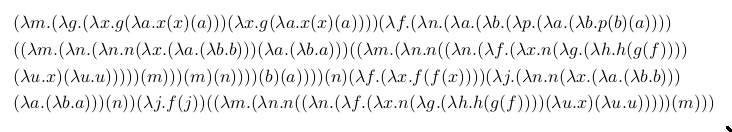
\includegraphics[width=16cm]{Images/oddevenlambda.png}
       \caption{Expanded lambda calculus function to determine the cardinality of a number.}
           \label{Fig:OddEvenLambda}
\end{figure}

With the ability to define any calculable function, Lambda Calculus is TC, as stated in the Church-Turing Thesis, Theorem \ref{thm:CTT}.
    \section{Proteus is Turing Complete}

This section will describe how we will construct 1+ proofs for showing that Proteus is TC.

\subsection{The Proteus Grammar}

List out the grammar and describe how it can be read, line by line.
Probably have a small example of a program that shows most of (maybe all) of the functionality with Proteus

\subsection{Initial Thoughts based off of the grammar}

List out some ideas that led to the idea that Proteus could be TC

\subsection{Proof Outline}

Theorems that would be used
Steps for proof outline

\subsection{Proof v1}

Formal proof that follows the outline

\subsection{Implementing Rule 110}

Implementation of Rule 110 that is a demonstration of TC.
    \section{Conclusion}

Succinctly describe what was the several techniques.
Compare and constrast them? Perhaps a discussion section?

    \newpage

    % references
    
    %alphabetical order
    %retrieval date is only for non-journal instances where material might change at a later date

    \begin{singlespace}

        \begin{thebibliography}{}

            \bibitem{NDTMeqDTM} Q. Gao and X. Xu, “The Analysis and Research on Computational Complexity,” pp. 3467–3472.

            \bibitem{GandyPaper} R. Gandy, “Church’s Thesis and Principles for Mechanisms,” The Kleene Symposium, pp. 123–148, Jun. 1980.

            \bibitem{ProteusRunTime} B. McClelland, “Adding Runtime Verification to the Proteus Language,” CSUN, May 2021.

            \bibitem{IntroFormLangAuto} P. Linz, An Introduction to Formal Languages and Automata. Jones \& Bartlett Learning, 2016.

            \bibitem{JavaGenericsTC} R. Grigore, “Java generics are turing complete,” ACM SIGPLAN Notices, vol. 52, no. 1, pp. 73–85, Jan. 2017, doi: https://doi.org/10.1145/3093333.3009871.

            \bibitem{MtGTC} A. Churchill, S. Biderman, and A. Herrick, “Magic: The Gathering is Turing Complete.”

            \bibitem{CivTC} A. de Wynter, “Turing Completeness and Sid Meier’s Civilization,” IEEE Transactions on Games, vol. 15, no. 2, pp.292-299, June 2023.

            \bibitem{GDLTC} A. Saffidine, “The Game Description Language Is Turing Complete,” IEEE Transactions on Computational Intelligence and AI in Games, vol. 6, no. 4, pp. 320–324, Dec. 2014, doi: https://doi.org/10.1109/tciaig.2014.2354417.

            \bibitem{CGoLTM} P. Rendell, "A Universal Turing Machine in Conway's Game of Life," 2011 International Conference on High Performance Computing \& Simulation, Istanbul, Turkey, 2011, pp. 764-772, doi: 10.1109/HPCSim.2011.5999906.
        
            \bibitem{TTTTM} S. S. T. Gontumukkala, Y. S. V. Godavarthi, B. R. R. T. Gonugunta and S. M., "Implementation of Tic Tac Toe Game using Multi-Tape Turing Machine," 2022 International Conference on Computational Intelligence and Sustainable Engineering Solutions (CISES), Greater Noida, India, 2022, pp. 381-386, doi: 10.1109/CISES54857.2022.9844404.

            \bibitem{ShallityAutomataThy} Jeffrey Outlaw Shallit, A second course in formal languages and automata theory. Cambridge ; New York: Cambridge University Press, 2009.

            \bibitem{JFLAPGrading} M. Biçer, F. Albayrak and U. Orhan, "Automatic Automata Grading System Using JFLAP," 2023 Innovations in Intelligent Systems and Applications Conference (ASYU), Sivas, Turkiye, 2023, pp. 1-4, doi: 10.1109/ASYU58738.2023.10296744.

            \bibitem{TuBB} E. Luce and S. H. Rodger, "A visual programming environment for Turing machines," Proceedings 1993 IEEE Symposium on Visual Languages, Bergen, Norway, 1993, pp. 231-236, doi: 10.1109/VL.1993.269602.
            
            \bibitem{LambdaCalcKleene} Dezani‐Ciancaglini Mariangiola and J. R. Hindley, “Lambda-Calculus,” Wiley Encyclopedia of Computer Science and Engineering, pp. 1–8, Sep. 2008, doi: https://doi.org/10.1002/9780470050118.ecse212.

            \bibitem{LambdaCalcRG} M. Dezani-Ciancaglini and J. R. Hindley, “Lambda-Calculus,” Nov. 2007, Available: \href{https://www.researchgate.net/publication/228107078_Lambda-Calculus}{https://www.researchgate.net/publication/228107078\_Lambda-Calculus}

            \bibitem{TutLambdaCalc} R. Rojas, “A Tutorial Introduction to the Lambda Calculus,” 2015, Available: \href{https://arxiv.org/pdf/1503.09060}{https://arxiv.org/pdf/1503.09060}

            \bibitem{AckermannPR} CWoo, “Ackermann function is not primitive recursive,” Mar. 2013, Available: \href{https://www.cs.tau.ac.il//~nachumd/term/42019.pdf}{https://www.cs.tau.ac.il//~nachumd/term/42019.pdf}
        
            \bibitem{RecursiveFuncs} W. Dean and A. Naibo, Recursive Functions, Fall 2024 Edition. Stanford University: Metaphysics Research Lab, Stanford University, 2024. Available: \href{https://plato.stanford.edu/archives/fall2024/entries/recursive-functions/}{https://plato.stanford.edu/archives/fall2024/entries/recursive-functions/}
        
            \bibitem{ChemTM} A. Hjelmfelt, E. D. Weinberger, and J. Ross, “Chemical implementation of neural networks and Turing machines.,” Proceedings of the National Academy of Sciences, vol. 88, no. 24, pp. 10983–10987, Dec. 1991, doi: https://doi.org/10.1073/pnas.88.24.10983.

            \bibitem{MCTM} “I Made a Working Computer with just Redstone!,” www.youtube.com. \href{https://www.youtube.com/watch?v=CW9N6kGbu2I}{https://www.youtube.com/watch?v=CW9N6kGbu2I}

            \bibitem{TerrariaTM} From Scratch, “I Made a 32-bit Computer Inside Terraria,” YouTube, Jun. 24, 2023. \href{https://www.youtube.com/watch?v=zXPiqk0-zDY}{https://www.youtube.com/watch?v=zXPiqk0-zDY}

            \bibitem{TerrariaTMGH} misprit7, "computerraria", Feb. 16, 2023, GitHub repository, \href{https://github.com/misprit7/computerraria}{https://github.com/misprit7/computerraria}
            
            \bibitem{nand2tetris} “Home | nand2tetris,” nand2tetris, 2017. \href{https://www.nand2tetris.org/}{https://www.nand2tetris.org/}

            \bibitem{ELTCompSys} Noam Nisan, ELEMENTS OF COMPUTING SYSTEMS : building a modern computer from first principles. 2020.

            % The above sources are the actual journals and books read/used in the thesis.
            % the below sources are just citations for declarations of info which are not explicitly journals or formal publications

            \bibitem{WolframRiceThm} Sakharov, Alex. “Rice’s Theorem.” From MathWorld--A Wolfram Web Resource, created by Eric W. Weisstein, Wolfram.com, 2024. \href{https://mathworld.wolfram.com/RicesTheorem.html}{https://mathworld.wolfram.com/RicesTheorem.html}
            
            \bibitem{WikiRiceThm} Wikipedia Contributors, “Rice’s theorem,” Wikipedia, Sep. 24, 2019. \href{https://en.wikipedia.org/wiki/Rice%27s_theorem}{https://en.wikipedia.org/wiki/Rice\%27s\_theorem}
            
            \bibitem{BfWiki} “Brainfuck,” Wikipedia, Oct. 05, 2021. \href{https://en.wikipedia.org/wiki/Brainfuck}{https://en.wikipedia.org/wiki/Brainfuck}
            
            \bibitem{BfGH} 262588213843476, “Basics of BrainFuck,” Gist, Oct. 29, 2024. \href{https://gist.github.com/roachhd/dce54bec8ba55fb17d3a}{https://gist.github.com/roachhd/dce54bec8ba55fb17d3a}

            \bibitem{BfSO} speeder, “How does the Brainfuck Hello World actually work?,” Stack Overflow, May 30, 2013. \href{https://stackoverflow.com/questions/16836860/how-does-the-brainfuck-hello-world-actually-work/19869651#19869651}{https://stackoverflow.com/questions/16836860/how-does-the-brainfuck-hello-world-actually-work/19869651\#19869651}
                        
            \bibitem{SmallestBfCompiler} “brainfuck - Esolang,” Esolangs.org, 2023. \href{https://esolangs.org/wiki/Brainfuck#Self-interpreters}{https://esolangs.org/wiki/Brainfuck\#Self-interpreters}
            
            \bibitem{SmallestBfCompilerActual} Brainfuck.org, 2024. \href{https://brainfuck.org/dbfi.b}{https://brainfuck.org/dbfi.b}
            
            \bibitem{GitMadeinC} “git.git - The core git plumbing,” Kernel.org, 2024. \href{https://git.kernel.org/pub/scm/git/git.git/tree/}{https://git.kernel.org/pub/scm/git/git.git/tree/}

            \bibitem{LinuxMadeinC} “kernel/git/torvalds/linux.git - Linux kernel source tree,” Kernel.org, 2024. \href{https://git.kernel.org/pub/scm/linux/kernel/git/torvalds/linux.git/tree/}{https://git.kernel.org/pub/scm/linux/kernel/git/torvalds/linux.git/tree/}

            \bibitem{GNUPreferC}  “Source Language (GNU Coding Standards),” Gnu.org, 2024. \href{https://www.gnu.org/prep/standards/html_node/Source-Language.html}{https://www.gnu.org/prep/standards/html\_node/Source-Language.html}
            
            \bibitem{MarketShareOS} StatCounter, “Desktop Operating System Market Share Worldwide | StatCounter Global Stats,” StatCounter Global Stats, 2019. \href{https://gs.statcounter.com/os-market-share/desktop/worldwide/}{https://gs.statcounter.com/os-market-share/desktop/worldwide/}
            
            \bibitem{COBOLBanks} “On the past, present, and future of COBOL – Increment: Programming Languages,” increment.com. \href{https://increment.com/programming-languages/cobol-all-the-way-down/}{https://increment.com/programming-languages/cobol-all-the-way-down/}

            \bibitem{CSUNStudents} “How Does California State University--Northridge Rank Among America’s Best Colleges?,” @USNews, 2015. \href{https://www.usnews.com/best-colleges/california-state-university-northridge-1153}{https://www.usnews.com/best-colleges/california-state-university-northridge-1153}

            \bibitem{JSPopular} H. Shah, “7 Frontend JavaScript Frameworks Loved by Developers in 2022,” Simform - Product Engineering Company, Feb. 17, 2022. \href{https://www.simform.com/blog/javascript-frontend-frameworks/}{https://www.simform.com/blog/javascript-frontend-frameworks/}

            \bibitem{ChatGPTPython} D. K. K. has years of experience as a S. D. S. H. enjoys coding, teaching, and has created this website to make M. L. accessible to everyone, “Is ChatGPT Written In Python??? [We FINALLY Found The Proof]» EML,” enjoymachinelearning.com, Feb. 09, 2023. \href{https://enjoymachinelearning.com/blog/is-chatgpt-written-in-python/}{https://enjoymachinelearning.com/blog/is-chatgpt-written-in-python/}

            \bibitem{RDataSci} Simplilearn, “What is R: Overview, its Applications and what is R used for | Simplilearn,” Simplilearn.com, Oct. 25, 2021. \href{https://www.simplilearn.com/what-is-r-article}{https://www.simplilearn.com/what-is-r-article}

            \bibitem{DataSciLangs} J. C. Luna, “Learn R, Python \& Data Science Online,” www.datacamp.com, Mar. 2023. \href{https://www.datacamp.com/blog/top-programming-languages-for-data-scientists-in-2022}{https://www.datacamp.com/blog/top-programming-languages-for-data-scientists-in-2022}

            \bibitem{vonNeumannImg} Kapooht, “English: von Neumann Architecture,” Wikimedia Commons, Apr. 28, 2013. \href{https://commons.wikimedia.org/wiki/File:Von_Neumann_Architecture.svg}{https://commons.wikimedia.org/wiki/File:Von\_Neumann\_Architecture.svg}

            \bibitem{HarvardArchImg} “File:Harvard architecture.svg - Wikimedia Commons,” Wikimedia.org, May 11, 2010. \href{https://commons.wikimedia.org/wiki/File:Harvard_architecture.svg}{https://commons.wikimedia.org/wiki/File:Harvard\_architecture.svg}

            \bibitem{4080Specs} “NVIDIA GeForce RTX 4080 Specs,” TechPowerUp, Oct. 13, 2023. \href{https://www.techpowerup.com/gpu-specs/geforce-rtx-4080.c3888}{https://www.techpowerup.com/gpu-specs/geforce-rtx-4080.c3888}

            \bibitem{IntelSpecs} “Intel® CoreTM i9-13900KS Processor (36M Cache, up to 6.00 GHz) - Product Specifications,” Intel. \href{https://www.intel.com/content/www/us/en/products/sku/232167/intel-core-i913900ks-processor-36m-cache-up-to-6-00-ghz/specifications.html}{https://www.intel.com/content/www/us/en/products/sku/232167/intel-core-i913900ks-processor-36m-cache-up-to-6-00-ghz/specifications.html}

            \bibitem{ALUImg} “File:2-bit ALU.svg - Wikibooks, open books for an open world,” Wikibooks.org, Oct. 18, 2011. \href{https://en.wikibooks.org/wiki/File:2-bit_ALU.svg}{https://en.wikibooks.org/wiki/File:2-bit\_ALU.svg}

            \bibitem{CellAutWiki} Wikipedia Contributors, “Cellular automaton,” Wikipedia, Dec. 05, 2019. \href{https://en.wikipedia.org/wiki/Cellular_automaton}{https://en.wikipedia.org/wiki/Cellular\_automaton}

            \bibitem{CellAutWolfram} E. W. Weisstein, “Cellular Automaton,” From Mathworld--A Wolfram Web Resource, mathworld.wolfram.com. \href{https://mathworld.wolfram.com/CellularAutomaton.html}{https://mathworld.wolfram.com/CellularAutomaton.html}

            \bibitem{CellAutBook} A. Ilachinski, Cellular Automata. World Scientific, 2001.

            \bibitem{CGoLImg} “Math’s ‘Game of Life’ Reveals Long-Sought Repeating Patterns | Quanta Magazine,” Quanta Magazine, Jan. 18, 2024. \href{https://www.quantamagazine.org/maths-game-of-life-reveals-long-sought-repeating-patterns-20240118/}{https://www.quantamagazine.org/maths-game-of-life-reveals-long-sought-repeating-patterns-20240118/}

            \bibitem{Rule110Img} “File:One-d-cellular-automaton-rule-110.gif - Wikimedia Commons,” Wikimedia.org, Nov. 20, 2018. \href{https://commons.wikimedia.org/wiki/File:One-d-cellular-automaton-rule-110.gif}{https://commons.wikimedia.org/wiki/File:One-d-cellular-automaton-rule-110.gif}

            \bibitem{CalcTC} Code \& Optimism, “How to write a Turing-Complete Programming Language in 40 minutes in Ruby using Bable-Bridge,” YouTube, Sep. 19, 2012. \href{https://www.youtube.com/watch?v=_Uoyufkb5lk}{https://www.youtube.com/watch?v=\_Uoyufkb5lk}

            \bibitem{CBfInter} M. Kenyon, “How to Write a Brainfuck Interpreter in C\#,” Thesharperdev.com, Oct. 12, 2019. \href{https://thesharperdev.com/how-to-write-a-brainfuck-interpreter-in-c/}{https://thesharperdev.com/how-to-write-a-brainfuck-interpreter-in-c/}

            \bibitem{MeepWebsite} “Compiling to Brainf\#ck - Meep.,” InJuly, 2024. \href{https://injuly.in/blog/bfinbf/index.html}{https://injuly.in/blog/bfinbf/index.html}

            \bibitem{MeepGH} srijan-paul, “GitHub - srijan-paul/meep: A programming language that compiles to brainfuck.,” GitHub, 2020. \href{https://github.com/srijan-paul/meep}{https://github.com/srijan-paul/meep}

            \bibitem{PythonBfInt} M. Ueding, “Creating a Brainfuck interpreter,” Martin Ueding, Apr. 19, 2023. \href{https://martin-ueding.de/posts/creating-a-brainfuck-interpreter/}{https://martin-ueding.de/posts/creating-a-brainfuck-interpreter/}

            \bibitem{FuncProgrChap} “Functional Programming,” learn.saylor.org. \href{https://learn.saylor.org/mod/book/tool/print/index.php?id=33044&chapterid=13087}{https://learn.saylor.org/mod/book/tool/print/\-index.php?id=33044\&chapterid=13087}

            \bibitem{LambdaCalcWiki} Wikipedia Contributors, “Lambda calculus,” Wikipedia, Jan. 02, 2020. \href{https://en.wikipedia.org/wiki/Lambda_calculus}{https://en.wikipedia.org/wiki/Lambda\_calculus}

            \bibitem{LambdaFuncsList} “Collected Lambdas,” jwodder.freeshell.org. \href{https://jwodder.freeshell.org/lambda.html}{https://jwodder.freeshell.org/lambda.html}

            \bibitem{SKICalcWiki} Wikipedia Contributors, “SKI combinator calculus,” Wikipedia, Oct. 28, 2024. \href{https://en.wikipedia.org/wiki/SKI_combinator_calculus}{https://en.wikipedia.org/wiki/SKI\_combinator\_calculus}

            \bibitem{RedditLambdaCalcPost} “Reddit - Dive into anything,” Reddit.com, 2017. \href{https://www.reddit.com/r/ProgrammerHumor/comments/78z90f/when_you_need_to_know_if_a_number_is_even_or_odd/}{https://www.reddit.com/r/ProgrammerHu\-mor/comments/78z90f/when\_you\_need\_to\_know\_if\_a\_number\_is\_even\_or\_odd/} 

            \bibitem{RedditLambdaCalcComment} “Reddit - Dive into anything,” Reddit.com, 2017. \href{https://www.reddit.com/r/ProgrammerHumor/comments/78z90f/comment/doylzry/}{https://www.reddit.com/r/ProgrammerHu\-mor/comments/78z90f/comment/doylzry/}

            \bibitem{TruncJava} “What is truncation in Java - Javatpoint,” www.javatpoint.com, 2021. \href{https://www.javatpoint.com/what-is-truncation-in-java}{https://www.javatpoint.com/what-is-truncation-in-java}

            \bibitem{TruncC} GeeksforGeeks, “trunc() , truncf() , truncl() in C language,” GeeksforGeeks, Jan. 25, 2018. \href{https://www.geeksforgeeks.org/trunc-truncf-truncl-c-language/}{https://www.geeksforgeeks.org/trunc-truncf-truncl-c-language/}

            \bibitem{ExcelTC} “The Excel Formula Language Is Now Turing-Complete,” InfoQ. \href{https://www.infoq.com/articles/excel-lambda-turing-complete/}{https://www.infoq.com/articles/excel-lambda-turing-complete/}

            \bibitem{AccTC} “Accidentally Turing-Complete,” beza1e1.tuxen.de. \href{https://beza1e1.tuxen.de/articles/accidentally_turing_complete.html}{https://beza1e1.tuxen.de/articles/accident\-ally\_turing\_complete.html}

            \bibitem{AccTC2} G. Branwen, “Surprisingly Turing-Complete,” gwern.net, Dec. 2012, Available: \href{https://gwern.net/turing-complete}{https://gwern.net/turing-complete}

            \bibitem{SecVuln} “A deep dive into an NSO zero-click iMessage exploit: Remote Code Execution,” Blogspot.com, 2021. \href{https://googleprojectzero.blogspot.com/2021/12/a-deep-dive-into-nso-zero-click.html?m=1}{https://googleprojectzero.blogspot.com/2021/12/a-deep-dive-into-nso-zero-click.html?m=1}

            \bibitem{ActorModelParallel} Wikipedia Contributors, “Actor model,” Wikipedia, Nov. 14, 2019. \href{https://en.wikipedia.org/wiki/Actor_model}{https://en.wikipedia.org/wiki/Actor\_model}
           
            \bibitem{ActorJavaParallel} L. Nigro, “Parallel Theatre: An actor framework in Java for high performance computing,” Simulation Modelling Practice and Theory, vol. 106, p. 102189, Jan. 2021, doi: https://doi.org/10.1016/j.simpat.2020.102189. 

            \bibitem{CartesianPlane} “Cartesian Plane - Definition, Meaning, Quadrants, Examples,” Cuemath. \href{https://www.cuemath.com/geometry/cartesian-plane/}{https://www.cuemath.com/geometry/cartesian-plane/}

            \bibitem{JavaUse1} “What Is Java Used For: 12 Real World Java Applications,” www.softwaretestinghelp.com. \href{https://www.softwaretestinghelp.com/real-world-applications-of-java/}{https://www.softwaretestinghelp.com/real-world-applications-of-java/}

            \bibitem{JavaUse2} “What is Java Used For?,” Codecademy News, Jun. 24, 2021. \href{https://www.codecademy.com/resources/blog/what-is-java-used-for/}{https://www.codecademy.com/resources/blog/what-is-java-used-for/}

            \bibitem{CPPUse1} Simplilearn, “Top 7 Practical Applications of C++ and the Way to Build a Career in the Field,” Simplilearn.com, Jan. 16, 2020. \href{https://www.simplilearn.com/c-plus-plus-programming-for-beginners-article}{https://www.simplilearn.com/c-plus-plus-programming-for-beginners-article}

            \bibitem{CPPUse2} “Uses of C++ | 10 Reasons Why You Should Use C++,” EDUCBA, Jul. 19, 2019. \href{https://www.educba.com/uses-of-c-plus-plus/}{https://www.educba.com/uses-of-c-plus-plus/}

            \bibitem{CPPFirefox} “mozilla/gecko-dev,” GitHub, Feb. 01, 2024. \href{https://github.com/mozilla/gecko-dev}{https://github.com/mozilla/gecko-dev}

            \bibitem{FirefoxMain} “The new, fast browser for Mac, PC and Linux | Firefox,” Mozilla, 2000. \href{https://www.mozilla.org/en-US/firefox/}{https://www.mozilla.org/en-US/firefox/}
        
            \bibitem{PHPScriptingServer} Astari S., “What Is PHP? Learning All About the Scripting Language,” Hostinger Tutorials, Apr. 30, 2019. \href{https://www.hostinger.com/tutorials/what-is-php/}{https://www.hostinger.com/tutorials/what-is-php/}

            \bibitem{PHPWP} http://facebook.com/syedbalkhi, “What is PHP? How PHP is Used in WordPress?,” WPBeginner, 2019. \href{https://www.wpbeginner.com/glossary/php/}{https://www.wpbeginner.com/glossary/php/}

            \bibitem{PHPLaravel} T. Otwell, “Laravel - The PHP Framework For Web Artisans,” Laravel.com, 2015. \href{https://laravel.com/}{https://laravel.com/}

            \bibitem{TopLangs1} L. dev, “Top 8 Most Demanded Programming Languages in 2023,” Devjobsscanner, Jun. 22, 2023. \href{https://www.devjobsscanner.com/blog/top-8-most-demanded-programming-languages/}{https://www.devjobsscanner.com/blog/top-8-most-demanded-programming-languages/}

            \bibitem{TopLangs2} L. Whitney, “Top 10 programming languages employers want in 2023,” TechRepublic, Feb. 03, 2023. \href{https://www.techrepublic.com/article/top-programming-languages-employers-want/}{https://www.techrepublic.com/article/top-programming-languages-employers-want/}

            \bibitem{TopLangs3} “11 of the Most In-Demand Coding Languages,” Indeed Career Guide. \href{https://www.indeed.com/career-advice/career-development/most-in-demand-coding-languages}{https://www.indeed.com/career-advice/career-development/most-in-demand-coding-languages}

            \bibitem{PyLibs} “Search results,” PyPI. \href{https://pypi.org/search/}{https://pypi.org/search/}

            \bibitem{NPM} npm, “npm | build amazing things,” Npmjs.com, 2019. \href{https://www.npmjs.com/}{https://www.npmjs.com/}

            \bibitem{Yarn} Yarnpkg.com, 2019. \href{https://yarnpkg.com/}{https://yarnpkg.com/}

            \bibitem{EasyLangs1} “10 Hardest and Easiest Programming Languages in 2024 - GUVI Blogs,” Mar. 01, 2023. \href{https://www.guvi.in/blog/easiest-programming-languages-to-hardest-ranked/}{https://www.guvi.in/blog/easiest-programming-languages-to-hardest-ranked/}

            \bibitem{EasyLangs2} “The 10 Most Popular Coding Languages to Learn in 2023 | BestColleges,” www.bestcolleges.com. \href{https://www.bestcolleges.com/bootcamps/guides/most-important-coding-languages/}{https://www.bestcolleges.com/bootcamps/guides/most-important-coding-languages/}

            \bibitem{FP1} J. M. Fernandes, “Functional Programming: With Examples and Lots of Cats,” Medium, Sep. 29, 2021. \href{https://medium.com/arctouch/thinking-functional-now-with-example-and-cats-8b9c2478b9af}{https://medium.com/arctouch/thinking-functional-now-with-example-and-cats-8b9c2478b9af}

            \bibitem{FP2} GeeksForGeeks, “Functional Programming Paradigm - GeeksforGeeks,” GeeksforGeeks, Jan. 02, 2019. \href{https://www.geeksforgeeks.org/functional-programming-paradigm/}{https://www.geeksforgeeks.org/functional-programming-paradigm/}

            \bibitem{RefTransp1} “Referential transparency,” Wikipedia, Jan. 05, 2021. \href{https://en.wikipedia.org/wiki/Referential\_transparency}{https://en.wikipedia.org/wiki/Referential\_transparency}

            \bibitem{RefTransp2} Claudiu, “What is referential transparency?,” Stack Overflow, Oct. 17, 2008. \href{https://stackoverflow.com/a/9859966}{https://stackoverflow.com/a/9859966}

            \bibitem{ElixirList} beam-community, “elixir-companies/priv/companies at main · beam-community/elixir-companies,” GitHub, 2015. \href{https://github.com/beam-community/elixir-companies/tree/main/priv/companies}{https://github.com/beam-community/elixir-companies/tree/main/priv/companies}

            \bibitem{HaskellListReadme} erkmos, “GitHub - erkmos/haskell-companies: A gently curated list of companies using Haskell in industry,” GitHub, 2017. \href{https://github.com/erkmos/haskell-companies?tab=readme-ov-file}{https://github.com/erkmos/haskell-companies?tab=readme-ov-file}

            \bibitem{ElixirListReadme} beam-community, “GitHub - beam-community/elixir-companies: A list of companies currently using Elixir in production.,” GitHub, 2015. \href{https://github.com/beam-community/elixir-companies}{https://github.com/beam-community/elixir-companies}

            \bibitem{HaskellList} “Haskell in industry - HaskellWiki,” Haskell.org, 2018. \href{https://wiki.haskell.org/Haskell\_in\_industry}{https://wiki.haskell.org/Haskell\_in\_industry}

            \bibitem{OCamlCoq} coq, “GitHub - coq/coq: Coq is a formal proof management system. It provides a formal language to write mathematical definitions, executable algorithms and theorems together with an environment for semi-interactive development of machine-checked proofs.,” GitHub, Sep. 04, 2024. \href{https://github.com/coq/coq?tab=readme-ov-file}{https://github.com/coq/coq?tab=readme-ov-file}

            \bibitem{ErlangUses} F. Cesarini, “Companies Who Use Erlang,” Erlang Solutions, Sep. 11, 2019. \href{https://www.erlang-solutions.com/blog/which-companies-are-using-erlang-and-why-mytopdogstatus/}{https://www.erlang-solutions.com/blog/which-companies-are-using-erlang-and-why-mytopdogstatus/}

            \bibitem{SimpleALU} “A Simple ALU, drawn from the ZipCPU,” zipcpu.com. \href{https://zipcpu.com/zipcpu/2017/08/11/simple-alu.html}{https://zipcpu.com/zipcpu/2017/08/11/simple-alu.html}

        \end{thebibliography}

    \end{singlespace}

    \appendix
    \addcontentsline{toc}{chapter}{Appendix}
        
    \chapter{Proof Assistants}\label{app:ProofAssist}

Initially, my goal was to learn how to use proof assistants to assert properties about Proteus.
I began to learn how to write basic and simple proofs using Coq.
Coq was powerful enough to show properties of systems that were publishable.
Whilst learning how to use Coq, I was learning to use TLA+ which proved equally as powerful, but not suited for my use case.
TLA+ is used for simultaneous computing as well as state machines which seemed very appealing upon initial inspection, since Proteus uses state machines as well.
However, this didn't extend well into demonstrating parts of Proteus that were not related to state machines.
I then considered using a different proof assistant like Dafny, Lean, or Twelf to see which would be better suited for proving something about Proteus.
I continued learning how to use the proof assistants and aimed to apply them to whatever proof I would eventually create about Proteus.

The big idea hit me one day; To show that Proteus was Turing Complete.
It was one of the biggest things to show in theory and was able to utilize all my knowledge and experience from this discipline.
There was only 1 problem, I couldn't use any proof assistant.
This is because fundamentally, it is impossible to show Turing Completeness using a proof assistant.

Recall Turing Completeness means that the shown system is equivalently as powerful as a TM, see section \ref{sec:TC}.
Also, recall the Church-Turing Thesis, Theorem \ref{thm:CTT}, which means that the definition of a TM is to be able calculate any calculable function.
Additionally, recall the proof of showing a system is TC in section \ref{subsubsec:NotableEgsFormalLang}.
The purpose of a proof assistant is to assert that the given proof is valid, step by step until the goal is reached.
Therefore for all inputs for any proof assistant, they are decidable (assuming they are well-written).
Thus, they are not capable of satisfying the Church-Turing Thesis, Theorem \ref{thm:CTT}, and also cannot be as powerful as a TM.
As such, it is impossible to use a proof assistant to show Turing Completeness.
This is when I abandoned using a proof assistant for proving Proteus TC.
    
    \chapter{Code Segments}\label{app:CodeSegments}

In this appendix section, I hope to put some of the larger code segments so that there is less interruption when reading the text.

\end{document}